\section{Introducció}
\label{cap:introduction}

En els darrers anys, l’ús d’aplicacions basades en \textit{blockchain} s’ha consolidat i ha donat lloc al que sovint s’anomena \textit{Web3}, és a dir, un conjunt d’aplicacions i serveis que permeten interactuar amb xarxes descentralitzades per transferir valor o executar lògica programable sense un control central únic \cite{ethereum_whitepaper,chainalysis_2024_trends}. En aquest context, el concepte de \textit{descentralització} fa referència a un model on el registre i la validació d’operacions no depèn d’una sola entitat, sinó d’una xarxa de participants; en contraposició, els sistemes \textit{centralitzats} deleguen la custòdia i el control a un intermediari (p. ex., una plataforma o un banc).

Una de les conseqüències d’aquest canvi és que l’usuari passa a gestionar directament els seus \textit{actius digitals} mitjançant una \textit{cartera digital} (\textit{wallet}), que és el programari que administra les claus criptogràfiques i permet autoritzar operacions a la xarxa \cite{ethereum_whitepaper}. Les aplicacions descentralitzades (\textit{DApps}) solen comunicar-se amb aquestes carteres a través d’una interfície estàndard al navegador. A la pràctica, això significa que quan l’usuari interactua amb una DApp, aquesta pot sol·licitar accions com l’enviament d’una \textit{transacció} (que no deixa de ser una operació que modifica l’estat a la \textit{blockchain} i pot implicar transferència de valor) o altres autoritzacions associades a contractes intel·ligents.

Tot i les oportunitats que ofereix aquest ecosistema, una problemàtica recurrent és que molts usuaris autoritzen operacions sense comprendre’n el contingut real. Aquest fenomen es coneix com a \textit{blind signing} (signatura a cegues): l’usuari aprova una operació sense disposar d’una descripció clara del que implica, sovint perquè la cartera només mostra dades tècniques o incompletes \cite{coinbase_blind_signing,ledger_blind_signing}. Aquesta manca de comprensió és especialment crítica quan la transacció inclou crides a contractes intel·ligents, ja que poden incorporar permisos persistents o accions complexes que no són evidents a simple vista.

Els informes de seguretat del sector assenyalen pèrdues econòmiques significatives associades a estafes, \textit{hacks} i explotacions en l’àmbit \textit{Web3}. Per exemple, Chainalysis estima que els fons robats a plataformes cripto van augmentar i van assolir xifres de l’ordre de milers de milions de dòlars en el darrer any analitzat \cite{chainalysis_stolen_2024,chainalysis_2025_report_intro}, i CertiK reporta pèrdues agregades també de diversos milers de milions en incidents \textit{on-chain} en el mateix període \cite{certik_hack3d_2024}. Aquestes dades reflecteixen que, més enllà dels atacs tècnics, una part del risc es materialitza en el moment en què l’usuari accepta una operació que no entén prou bé.

Davant d’aquest escenari, es fa necessari disposar d’eines que augmentin la transparència i la comprensió en el pas previ a la confirmació. En aquest sentit, les carteres digitals poden esdevenir un punt d’intervenció especialment rellevant, ja que constitueixen l’espai on l’usuari acaba validant l’operació. Més concretament, MetaMask incorpora un sistema de funcionalitats addicionals, anomenat \textit{MetaMask Snaps}, que permet estendre el comportament de la cartera i desenvolupar mecanismes capaços d’aportar context, explicacions i \textit{transaction insights} abans que l’usuari signi \cite{metamask_tx_insights,metamask_entrypoints,metamask_permissions,consensys_snaps_launch}.

En aquest treball es proposa i s’implementa un assistent de seguretat integrat com a Snap, capaç d’interceptar transaccions abans de la confirmació, analitzar-les mitjançant regles deterministes per identificar patrons de risc i generar explicacions en llenguatge natural. L’objectiu és reduir la signatura a cegues i facilitar decisions informades, mantenint la privadesa mitjançant execució local dels components d’anàlisi i d’explicació.

\subsection{Objectius}

L’objectiu principal d’aquest treball és dissenyar i implementar un sistema capaç d’assistir l’usuari durant el procés de signatura de transaccions en entorns Web3, proporcionant informació clara sobre les implicacions de cada acció abans de la seva confirmació.

Per assolir aquest objectiu general, el projecte planteja diverses fites específiques. En primer lloc, desenvolupar un mecanisme d’interceptació de transaccions que permeti analitzar-les abans que siguin executades. En segon lloc, implementar un sistema d’anàlisi capaç de detectar patrons potencialment perillosos associats a autoritzacions excessives o operacions de risc elevat. En tercer lloc, generar explicacions en llenguatge natural que tradueixin la informació tècnica a un format comprensible per a usuaris no especialitzats. Finalment, validar el sistema en un entorn de proves realista que permeti avaluar-ne el comportament, el rendiment i les limitacions.


El projecte es concep com una solució modular i extensible, amb la voluntat de servir com a base per a futures ampliacions i millores en l’àmbit de la seguretat i l’explicabilitat (és a dir, la capacitat d’explicar de manera clara i entenedora per què una transacció pot ser arriscada i què implica) en aplicacions descentralitzades.

\newpage

\subsection{Justificació}

L’ecosistema \textit{blockchain} i el mercat dels actius digitals han experimentat un creixement sostingut durant els darrers anys. Segons dades de Triple-A, l’any 2024 el nombre de persones que posseïen criptomonedes al món superava els 560 milions, amb un increment interanual del 34\% respecte de 2023 \cite{triplea_ownership_2024}. Aquest augment fa que cada vegada més usuaris accedeixin a serveis basats en \textit{blockchain} sense una formació tècnica específica, fet que incrementa la probabilitat d’errors d’interpretació i les decisions poc informades en el moment de signar operacions.

Aquest increment d’adopció no només amplia l’ús de les tecnologies descentralitzades, sinó també la seva superfície d’exposició al risc. Informes recents de Chainalysis i CertiK mostren que les pèrdues associades a robatoris, estafes i explotacions dins l’ecosistema cripto continuen assolint xifres molt elevades, amb milers de milions de dòlars compromesos anualment \cite{chainalysis_stolen_2024,chainalysis_2025_report_intro,certik_hack3d_2024}. En molts casos, aquests incidents no depenen únicament d’un error tècnic del protocol, sinó també del fet que l’usuari autoritza transaccions o permisos sense entendre amb precisió què impliquen.

Aquesta situació posa en evidència una mancança important en les eines actuals d’interacció amb Web3. Tot i que existeixen solucions comercials orientades a la detecció de riscos, moltes basen el seu funcionament en serveis externs, criteris de classificació opacs o avisos genèrics que adverteixen, però no expliquen \cite{metamask_tx_insights,consensys_snaps_launch}. Això limita la capacitat de l’usuari per comprendre el motiu real del risc i, en conseqüència, per prendre decisions informades. En aquest sentit, la proposta es justifica no sols per la necessitat de reforçar la seguretat, sinó també per la d’augmentar la comprensió i la transparència en el procés de signatura de transaccions.

A partir d’aquest context, el treball se centra en tres eixos principals: privadesa, explicabilitat i transparència. La privadesa s’entén com la voluntat de minimitzar l’exposició de dades sensibles a tercers; l’explicabilitat, com la capacitat del sistema d’indicar no només si una acció pot ser arriscada, sinó també per què ho és d’una manera clara i comprensible; i la transparència, com l’ús de criteris d’avaluació entenedors i auditables.

Des d’un punt de vista acadèmic, aquest sistema resulta rellevant perquè combina àmbits d’interès actual com la seguretat informàtica, les aplicacions descentralitzades i la intel·ligència artificial aplicada. A més, es planteja dins un marc tècnicament viable, basat en eines de codi obert, entorns de prova públics i una arquitectura modular que permet abordar el problema de manera progressiva. Aquest plantejament fa possible desenvolupar una solució funcional amb recursos assumibles, alhora que obre la porta a futures ampliacions i línies de treball posteriors.


\newpage

\subsection{Planificació}
\label{sec:planificacio}

La planificació del projecte s’ha plantejat de manera progressiva al llarg de diversos mesos, des de la fase inicial d’anàlisi fins a la redacció final de la memòria. Atès que es tracta d’un treball amb una forta component pràctica i d’investigació, l’organització temporal no s’ha orientat a una execució estrictament lineal, sinó a una evolució per fases que permeti avançar de forma incremental.

En una primera etapa s’ha previst la definició del problema, l’estudi del context tecnològic i la identificació de les necessitats que justifiquen la proposta. A continuació, es planteja una fase centrada en el disseny del sistema i la definició dels seus components principals. Posteriorment, es preveu el desenvolupament del prototip i la integració dels diferents elements necessaris per al seu funcionament. Finalment, el procés es completa amb la validació experimental, l’anàlisi dels resultats i la preparació de la documentació definitiva.


\begin{figure}[H]
    \centering
    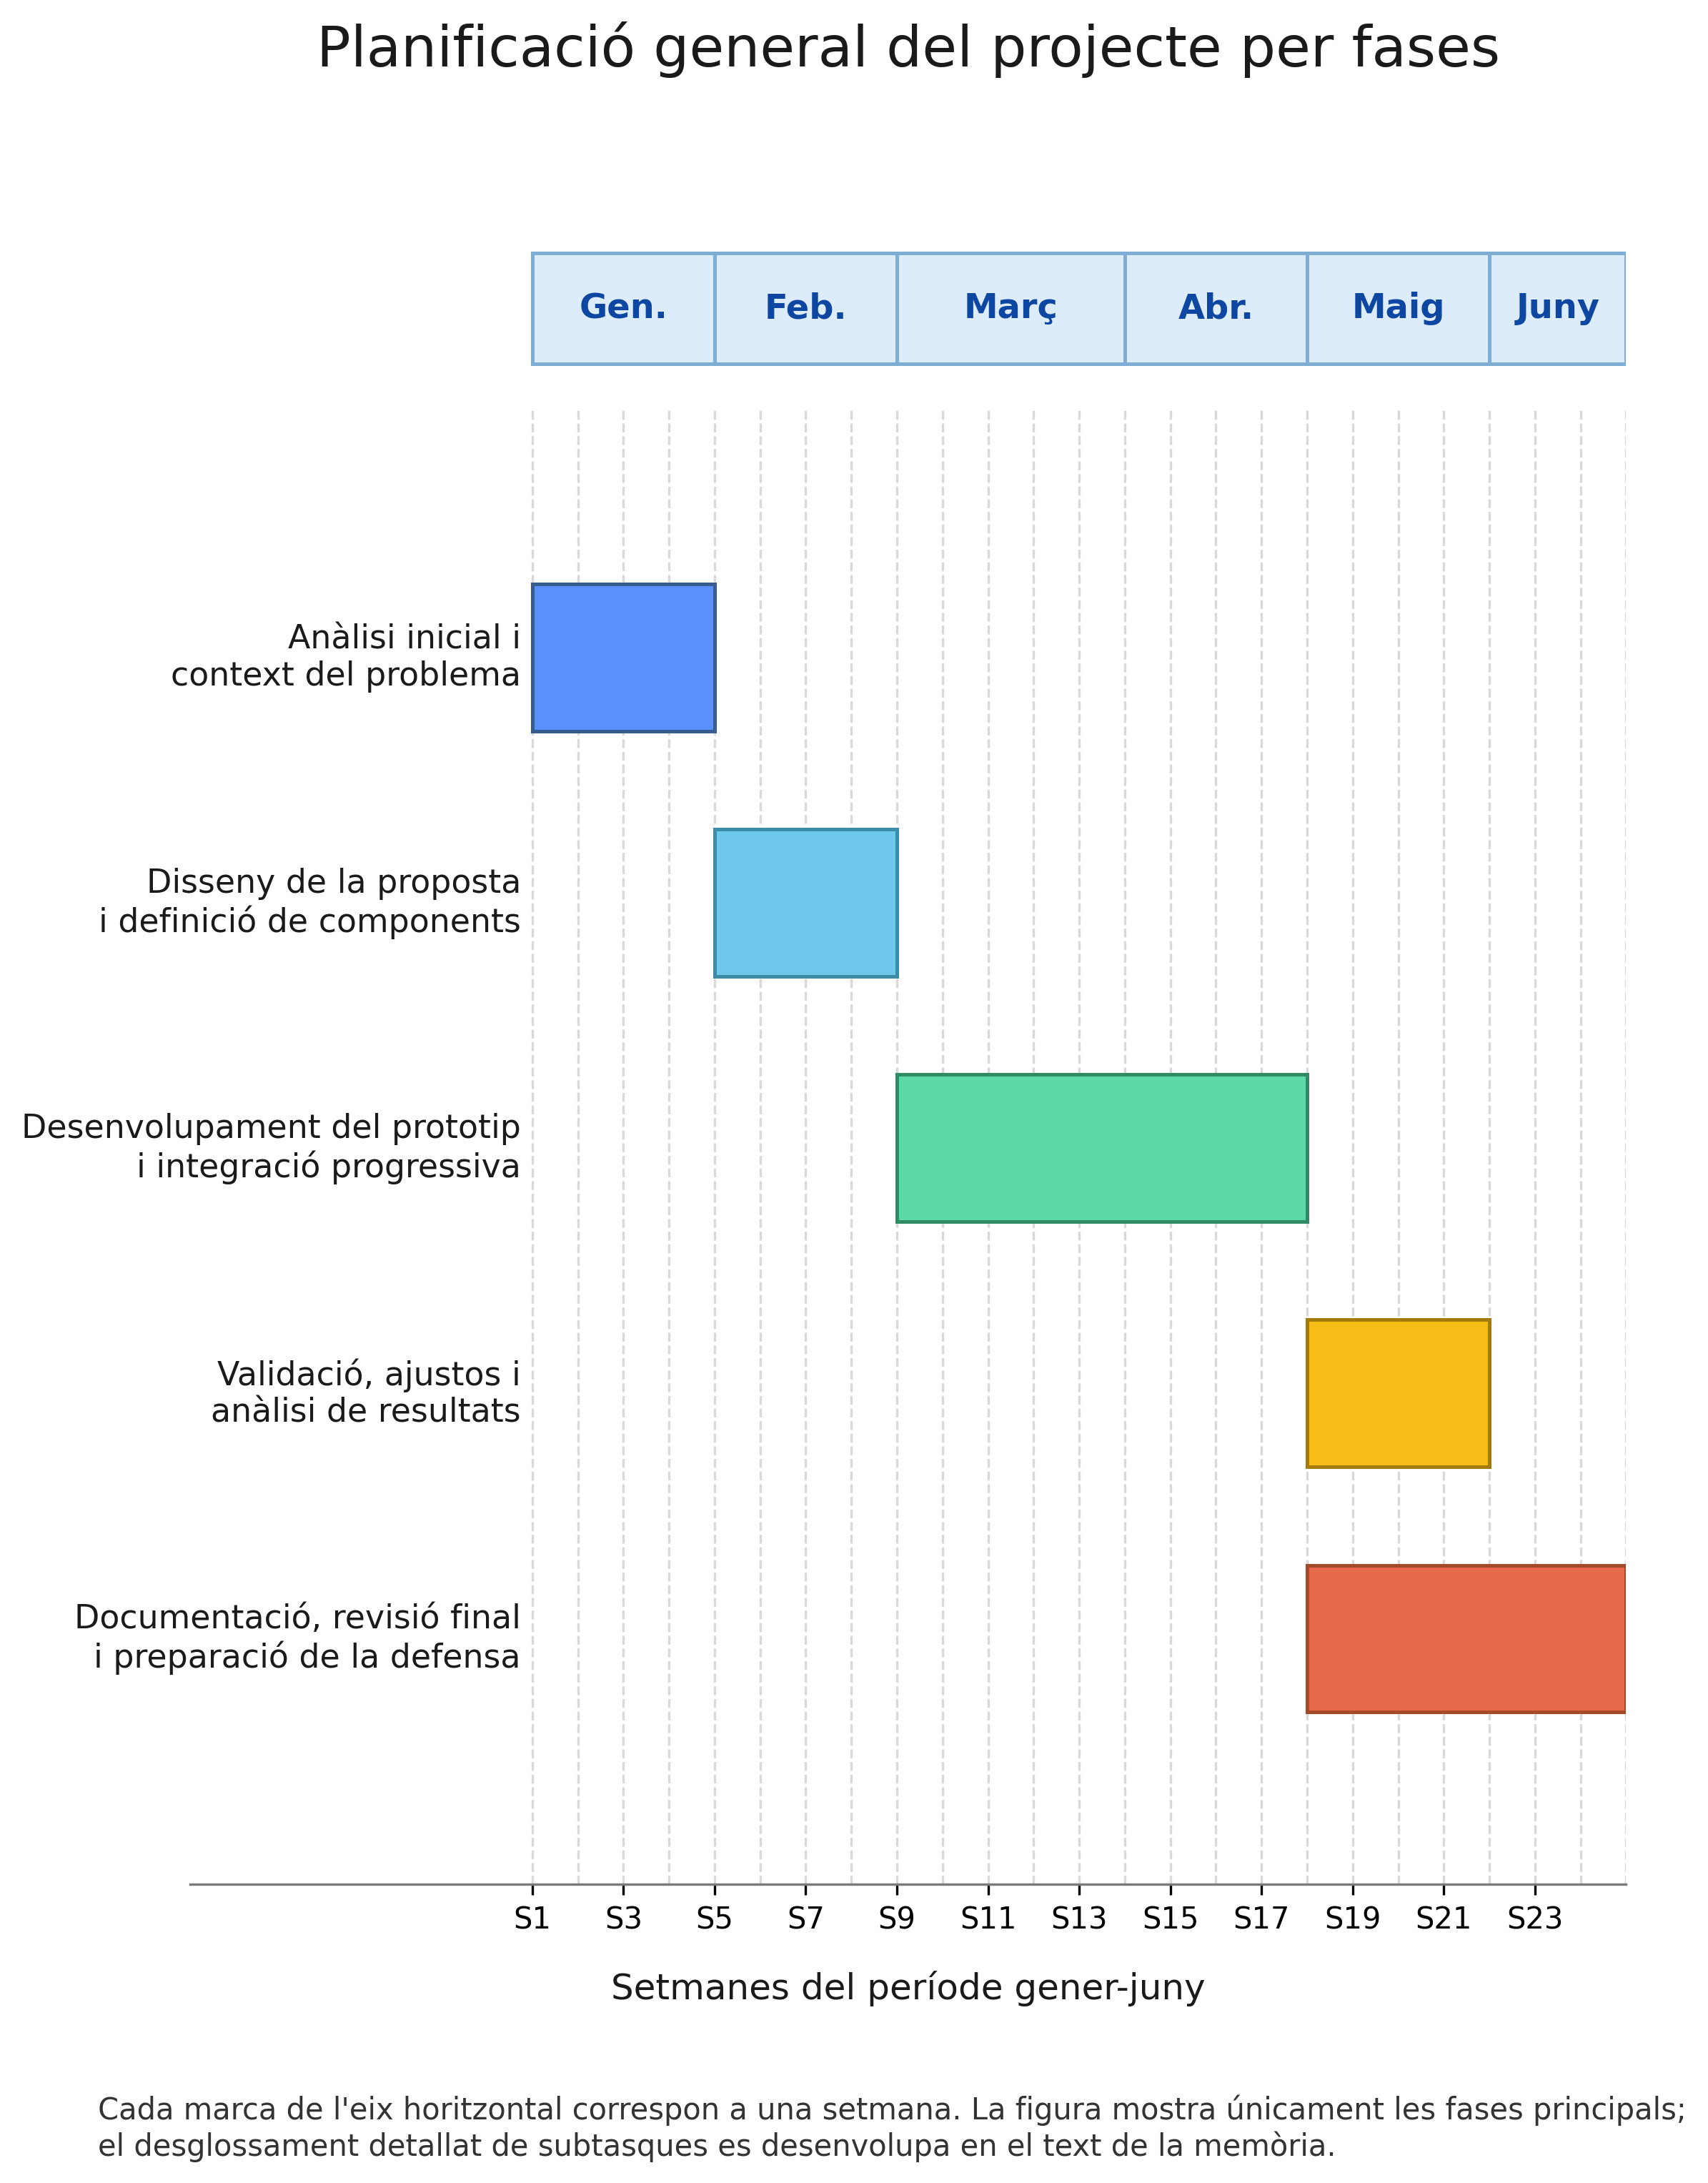
\includegraphics[width=0.70\textwidth]{imgs/gantt_generic_tfg.png}
    \caption{Planificació general del projecte per fases}
    \label{fig:gantt-general-fases}
\end{figure}

La Figura~\ref{fig:gantt-general-fases} mostra la planificació general del projecte distribuïda en fases principals. Per facilitar-ne la lectura, el diagrama s’ha simplificat a un nivell macro, mentre que el detall de subtasques i activitats específiques es descriu en el text. Cada marca de l’eix horitzontal correspon a una setmana del període comprès entre gener i juny.

\newpage

Des d’un punt de vista organitzatiu, aquesta planificació permet distingir clarament entre les fases de comprensió del problema, definició de la proposta, desenvolupament, validació i tancament. Tot i això, cal tenir en compte que en un projecte d’aquestes característiques poden aparèixer iteracions entre fases, especialment entre el disseny, la implementació i les proves. Per aquest motiu, el diagrama s’ha d’interpretar com una previsió orientativa que estructura el treball i en facilita el seguiment, més que no pas com una seqüència rígida i tancada.

 

% Aquesta secció inclourà el diagrama de Gantt amb la descomposició de tasques quan el projecte estigui més avançat
% Inclourà:
% - Descomposició de tasques principals
% - Estimació temporal per a cada fase
% - Diagrama de Gantt amb les dependències
% - Fites principals del projecte


\subsection{Organització de la memòria}

La memòria s’estructura en sis capítols que presenten de manera progressiva el context, el disseny, la implementació i l’avaluació del sistema desenvolupat.

El Capítol~\ref{cap:general_description} proporciona el context tecnològic necessari per comprendre la proposta: Web3, blockchain, Ethereum, contractes intel·ligents, carteres digitals i MetaMask Snaps. També hi revisa algunes solucions de seguretat existents i els elements diferenciadors del sistema proposat.

El Capítol~\ref{cap:design} presenta el disseny de la proposta. S’hi defineixen els requisits funcionals i no funcionals, els actors, l’arquitectura general, el flux de comunicació i els casos d’ús principals, i s’hi justifiquen les decisions de disseny adoptades.

El Capítol~\ref{cap:implementation} descriu la implementació tècnica del prototip: l’entorn d’execució, la DApp local, el Snap, el backend d’anàlisi, la base de dades local i la integració amb Ollama.

El Capítol~\ref{cap:evaluation} se centra en l’avaluació. S’hi descriu l’estratègia i el protocol de proves, es presenten els escenaris amb els resultats observats i s’analitza la capacitat de classificació mitjançant una matriu de confusió, juntament amb el grau de compliment dels requisits.

El Capítol~\ref{cap:conclusions} valora l’assoliment dels objectius, resumeix els resultats i els problemes detectats, proposa línies de treball futur i inclou una reflexió sobre els aspectes ètics, socials i ambientals. Finalment, la memòria incorpora les referències bibliogràfiques utilitzades durant el desenvolupament.











% Aquesta secció es completarà al final, un cop definits tots els capítols
% Descriurà l'estructura dels capítols següents:
% - Capítol 2: Background (tecnologies i estat de l'art)
% - Capítol 3: Disseny de la proposta
% - Capítol 4: Implementació
% - Capítol 5: Avaluació
% - Capítol 6: Conclusions i treball futur
